\chapter{Project Management}
\section{Terms}
Here follows a description of terms that are useful to understand how the project management functioned. 

\begin{description}
\item[Scrum] \label{def:scrum}is an popular agile software development methodology. This means that the work is done in increments called sprints, and daily meetings are held to update the rest of the team on progress and problems. The scrum process also has roles for team members, in particular a team member called scrum master who handles contact between the development team and people outside the team.

\item[Sprint] \label{def:sprint} is a period in which work is planned and done. It has a duration of one week. At the end of each sprint the group is updated on progress achieved, and sets goals for the next sprint. 
\item[Kanban-board] \label{def:kanban} is a visual aid that was used to display work packages, with content, people assigned to each package, and status of work package (to do, currently worked on, finished). The intent was to simplify and organize the work being done and work in need of finishing.
\end{description}
\section{Development process}

The customer favored the use of an iterative approach to the development process, where every sprint added a new layer of functionality, either to the application or the underlying model. Each sprint lasted for a period of 1-2 weeks, and the exact content was worked out in collaboration with the customer. Short term plans were favored over longer plans, due to the flexibility provided. While this made formulating definite goals for the final product difficult, the customer and the group were in agreement that due to the research intensive nature of the project, a high degree of flexibility was required. 

It was decided that the developers would have online meetings twice a week and an offline meeting once a week. 
The working hours were set to not less than 20 hours a week, but the developers were free to choose when to work themselves. This number was the expected workload for the course, and made a reasonable target for work per week. The meetings with the team was set to two times per week instead of once per day, so it could fit with the schedules of the team members. This was different from other agile methods like Scrum, but if was a necessary adaptation to fit meetings into the entire teams schedule. Updates were shared among the team members with email, trello\footnote{See \pageref{def:trello} for more info}, and it's learning as a replacement for daily meetings.

\section{Plans}

Nearing the end of every sprint, the customer and group agreed upon the content of the following sprint. This list has been placed in Figure \ref{tab:sprintList}, and provided a short summary of what was accomplished in a particular time-frame. 


\section{Team Roles and Organization}
There was not much place for specific roles among the group, as it was a small group, and the project required that all the members were capable and willing to work at all the tasks. This makes a difference from development models with specific roles and tasks assigned. Roles that were set for the group were therefore mainly organizers, so that one person was to keep awareness of what work needed to be completed in a particular domain, and share it with the rest of the group:

\begin{description}

\item[Group Leader] Elias was made organizer, and got the responsibilities of reminding the group of what to do.
\item[Document-organizer] Johannes was tasked with organizing documentation and distributing the work of writing the report to the group. 
\end{description}

\section{Comparison}
The development model used by the group was a form of agile development. Other well-known examples of agile methodologies were scrum and extreme programming. 

\section{Management Tools}
 
\begin{description}

\item[Trello]  \label{def:trello} was a collaboration tool with the ability to create interactive kanban-boards online. This use of this tool was to allow the group to coordinate tasks that were to be done, and the progress on the tasks, and which members were to work on which task. 
\item[It's learning] was used to distribute information that was not time -critical, with a message board being used. It's learning would not send messages when a new topic or message appeared, so it's use for time-critical messages or making sure that everyone would read it was limited. 
\item[Email] was used for time-critical communication, and for information that needed feedback swiftly, often within the same day.
\item[Github] \label{def:github} was used to share code, and to describe and mark issues found in the code when problems were discovered. The relevant issues could then be discussed on the website
\end{description}
\section{Work Breakdown Structure}
With a development methodology that stresses short term goals, it is only possible to plan WBS for the current period. After the customer has specified the goal for the following week, we immediately sat down and defined the WBS for the given period. This was, a WBS was developed incrementally by adjoining the new WBS to the previous. The WBS was made in graphical form, as can be seen in Figure \ref{fig:WBS}.

\begin{figure}[p]

\setlength\fboxsep{0pt}
\setlength\fboxrule{1pt}\noindent\makebox[\textwidth]{%
 \fbox{
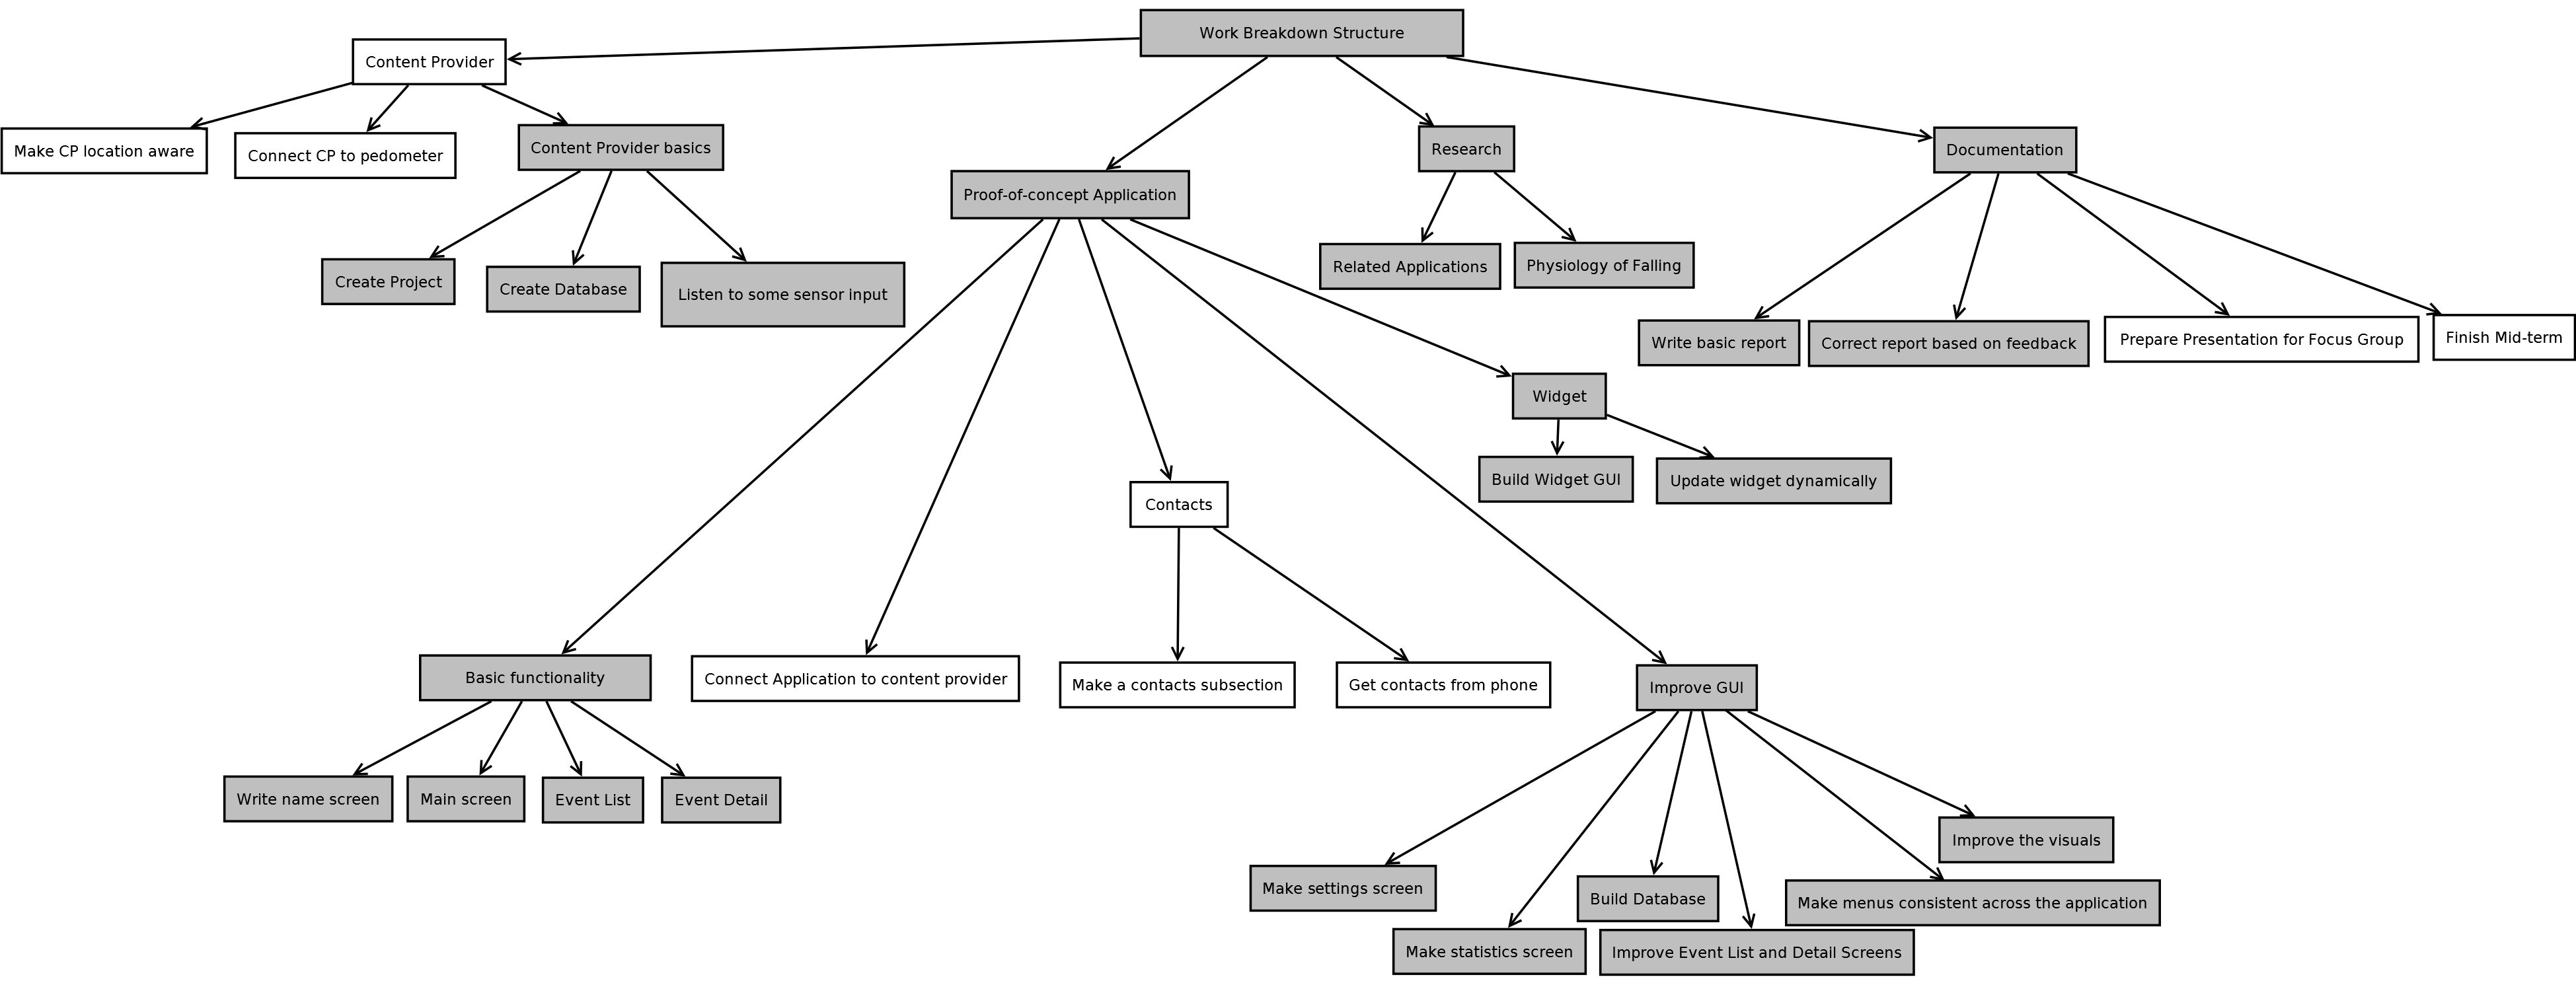
\includegraphics[width=1.45\textwidth , angle=270]{Res/WBS15313.png}
}
}
\label{fig:WBS}
\caption{The current WBS}
\end{figure}